% Created 2024-11-03 Sun 16:51
% Intended LaTeX compiler: pdflatex
\documentclass[12pt]{article}
\usepackage[utf8]{inputenc}
\usepackage[T1]{fontenc}
\usepackage{graphicx}
\usepackage{longtable}
\usepackage{wrapfig}
\usepackage{rotating}
\usepackage[normalem]{ulem}
\usepackage{amsmath}
\usepackage{amssymb}
\usepackage{capt-of}
\usepackage{hyperref}
\usepackage[margin=1in]{geometry} \usepackage{amsmath}
\author{Jason Press}
\date{\today}
\title{Pondering Pendulums}
\hypersetup{
 pdfauthor={Jason Press},
 pdftitle={Pondering Pendulums},
 pdfkeywords={},
 pdfsubject={},
 pdfcreator={Emacs 29.4 (Org mode 9.7.11)}, 
 pdflang={English}}
\begin{document}

\maketitle
\begin{abstract}
In this lab, we derived the equation for the period of a pendulum by varying the mass, string length, and initial angle of a pendulum. To do this, we changed one variable of the system and then measured the period of the pendulum. From this, we can create a relationship between the change in period versus change of the quantity in one mass. We discovered that \(T = km^al^b\theta^c\) where \(k = 2.0314\pm0.0139\), \(a = 0.002646\pm0.001254\), \(b = 0.4730\pm0.0058\), and \(c = 0.0054\pm0.0021\).
\end{abstract}
\section{Introduction}
\label{sec:org265789b}

In this lab, we measured varying properties of a pendulum system to determine the factors that impact the period of a pendulum. In a gravity pendulum with a massless string, there are three possible factors to vary: the mass at the end \(m\), the length of the string \(l\), and the initial angle \(\theta\). Thus we derive the following equation for the period \(T\) expressed with constants \(k\), \(a\), \(b\), and \(c\):

\begin{align}\label{eq:hypo}
T = km^al^b\theta^c
\end{align}

In order to derive \(a\), \(b\), and \(c\), we can use properties of logarithms to get the following equation:

\begin{align}
\ln T = \ln k + a \ln m + b \ln l + c \ln \theta
\end{align}

Thus, if we only change one variable, we can create linear relationships to derive the constants \(a\), \(b\), and \(c\) for their respective variable. Using our derived constants, we can rearrange Equation \ref{eq:hypo} to solve for \(k\):

\begin{align}\label{eq:k}
k = \frac{T}{m^a l^b \theta^c}
\end{align}
\section{Methods}
\label{sec:orgf8875db}

Our pendulum consisted of a protractor with a piece of light fishing line, with a loop on the bottom to attach weights. We attached the protractor to a vertical pole, such that we could easily change the height of the protractor. We attached a horizontal beam through the marked center of the protractor, and then attached the fishing line to the beam. We tied a large loop at the bottom of the fishing line. All of our weights had a hole through the center, so all we had to do to attach the weight to the end of the line was thread the loop through the hole of the weight, and then loop the line back on itself across the weight. With that, we had a complete pendulum.

To measure the period, we adjusted the height of the pendulum such that the weight would pass through a photogate that would measure the period of the pendulum.

To change the mass of the pendulum, we put a new weight on the pendulum, while keeping the length and release angle constant. All of our masses were the same size, so the overall length of the pendulum did not change. To measure the mass of the pendulum, we assumed the mass of the fishing line was negligible compared to the mass on the end, so we just measured the mass of the mass.

To change the length of the string of the pendulum, we wrapped the pendulum around the horizontal beam more or less to get a shorter or longer length. To measure the length of the string, we used a meterstick, starting from the top of the mass and ending at the bottom of the beam, where the string could freely pivot. As long as we measured the length of the string the same way across all of the trials, we would get consistent answers, since changing the starting point (i.e. measuring from the bottom of the mass instead of the top of the mass) would change the y-intercept of the regression of \(T\) versus \(a \ln l\), and not change the slope.

To change the initial angle of the pendulum, we released it from a different angle. To get the angle, we pulled the mass from equilibrium until the desired gradient mark, and then released the mass from rest.

We used three different weights, five different string lengths, and five different initial angles to get our linear relationship with \(T\) for the respective variable.

\begin{center}
\includegraphics[width=6.5in]{./setup.png}
\captionof{figure}{Pendulum setup}
\end{center}
\section{Results}
\label{sec:orge50f4b8}

Here are our results for varying \(m\) with \(l = 0.515\)m and \(\theta = 0.3491\) radians:

\begin{table}[htbp]
\caption{\(m\) versus \(T\)}
\centering
\begin{tabular}{c|c}
\(m\) (kg) & \(T\) (s)\\
\hline
0.0653 & 1.4690\\
0.0710 & 1.4700\\
0.0935 & 1.4706\\
\end{tabular}
\end{table}

The resulting slope of \(\ln T\) versus \(\ln m\) is 0.002646\textpm{}0.001254.

\begin{center}
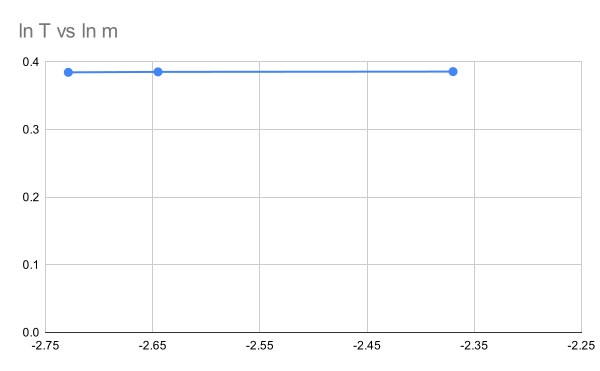
\includegraphics[width=6.5in]{./tvm.pdf}
\captionof{figure}{\(\ln T\) versus \(\ln m\)}
\end{center}

Here are our results for varying \(l\) with \(m = 0.0710\)kg and \(\theta = 0.3491\) radians:

\begin{table}[htbp]
\caption{\(l\) versus \(T\)}
\centering
\begin{tabular}{c|c}
\(l\) (m) & \(T\) (s)\\
\hline
0.515 & 1.4700\\
0.399 & 1.2968\\
0.318 & 1.1600\\
0.274 & 1.0800\\
0.154 & 0.8300\\
\end{tabular}
\end{table}

The resulting slope of \(\ln T\) versus \(\ln l\) is 0.4730\textpm{}0.0058.

\begin{center}
\includegraphics[width=6.5in]{./tvl.pdf}
\captionof{figure}{\(\ln T\) versus \(\ln l\)}
\end{center}

Here are our results for varying \(\theta\) with \(m = 0.0710\)kg and \(l = 0.438\)m:

\begin{table}[htbp]
\caption{\(\theta\) versus \(T\)}
\centering
\begin{tabular}{c|c}
\(\theta\) (radians) & \(T\) (s)\\
\hline
0.44 & 1.3610\\
0.35 & 1.3590\\
0.26 & 1.3500\\
0.17 & 1.3510\\
0.09 & 1.3489\\
\end{tabular}
\end{table}

The resulting slope of \(\ln T\) versus \(\ln \theta\) is 0.0054\textpm{}0.0021.

\begin{center}
\includegraphics[width=6.5in]{./tvt.pdf}
\captionof{figure}{\(\ln T\) versus \(\ln \theta\)}
\end{center}

Using Equation \ref{eq:k}, we get an average \(k = 2.0314\pm0.0139\).
\section{Discussion}
\label{sec:org03fa51b}

Overall, our \(k\) is very close to \(\frac{2\pi}{\sqrt{g}} = 2.0061\). The sources of statistical errors in this lab come from non-conservative forces: there is a small amount of air resistance, friction in the string, the string does not have zero mass. All of these factors combine to give a constant of \(b\) that is slightly smaller than it should be.

Given that \(a\) and \(c\) are (for all intents and purposes) zero, the only source of systematic error that impacted our results was from measuring \(l\). Whenever we measured one variable, we kept the other two the same. For example, whenever we measured \(l\), even if our \(\theta\) was not exactly 0.3419 radians, we kept it at the same \(\theta\) measured by the protractor. Having a \(\theta\) that is not perfect does not matter, because the slope of \(\ln l\) versus \(\ln T\) is only affected by relative changes.
\section{Sample Calculations}
\label{sec:org4ac2d24}

We used a spreadshet for all of our calculations. To get the ln of a value, we did \texttt{=ln(B2)} for cell \texttt{B2}, repeat for all relevant data values. Then, to get the slope of a system, we used the \texttt{LINEST(ln(times), ln(variables), true, true)} function to get the slope and error. Then, we calculated \(k\) with each individual data point; for example, \texttt{=E2/B2\textasciicircum{}B12/C2\textasciicircum{}H13/D2\textasciicircum{}N13}. Then, to get an average value for \(k\) over all thirteen trials, we used the average of all the values, i.e. \texttt{=AVERAGE(B19:B21,H20:H24,N20:N24)}. To get the average error, we took a weighted sum of squares, i.e. \texttt{=sqrt(3*B13\textasciicircum{}2+5*H14\textasciicircum{}2+5*N14\textasciicircum{}2)}. This is the spreadsheet we used:

\begin{center}
\includegraphics[width=6.5in]{./spreadsheet.png}
\end{center}

For the graphs, we used the ln of the variables, chose the ln(T) section to be the y-axis, and the ln(variable) section to be the x-axis.
\end{document}
